\documentclass[usenames,dvipsnames]{beamer}
\usetheme{Berlin}
\usepackage[utf8]{inputenc}
\usepackage[english]{babel}
\usepackage{graphicx}
\usepackage{url}
\usepackage{multicol}
\usepackage{relsize}

\graphicspath{ {images/} }

\title{Secure memory handling in C}
\subtitle{}
\author{Alexander Livenets\\Oliver Esser}
\institute{}
\date{25 June 2019}

\newcommand{\codeinline}[1] {\texttt{\smaller[2]{#1}}}

\begin{document}

\AtBeginSection[]
{
\begin{frame}
\frametitle{Table of Contents}
\tableofcontents[currentsection]
\end{frame}
}

\setbeamertemplate{endpage}{%
\begin{frame}
\center \Huge Thanks!
\end{frame}
}

\begin{frame}
\titlepage
\end{frame}

\section{Memory handling}
\begin{frame}
\frametitle{Buffer overflow example}
% \begin{verbatim}
% int copy_string(const char *s)
% {
% 	char buffer[64];
% 	strcpy(buffer, s);
% }

% int main(void)
% {
% 	char larte_string[128] = "Hello World!";
% 	copy_string(large_string); //OK...

% 	// Fill large string
% 	for(int i = 0; i < sizeof(large_string) - 1; ++i)
% 		large_string[i] = 'a';
% 	large_string[sizeof(large_string) - 1] = '\0';

% 	copy_string(large_string); // Buffer overflow...
% }
% \end{verbatim}
\note{When string on stack overflows, return address or other sensitive data on stack may be corrupted, hence allowing to perform attack}
\end{frame}

% \begin{frame}
% \centering
% 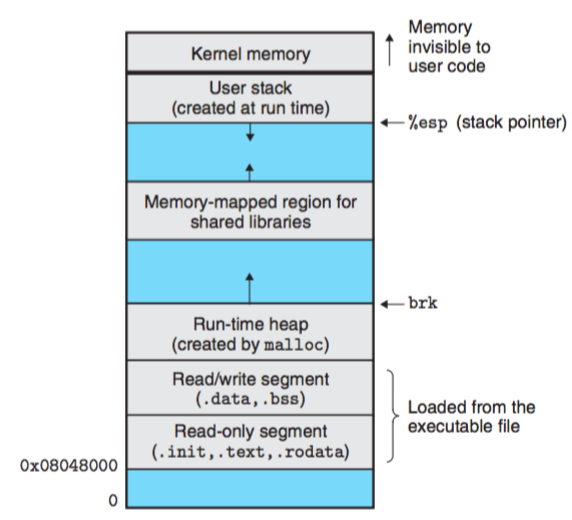
\includegraphics[scale=0.35]{linux_mem.png}
% \tiny{https://people.cs.pitt.edu/~xianeizhang/notes/Linking.html}
% \end{frame}

% \begin{frame}
% \note{Show results of buffer overflow: return address may be overwritten and function will return to the malicious address}
% \end{frame}
% \section{strcpy family}
% \begin{frame}
% TODO
% \end{frame}

% \section{sprintf family}
% \begin{frame}
% TODO
% \end{frame}

% \section{Memory handling in C++}
% \begin{frame}
% \frametitle{\secname}
% TODO
% \end{frame}

\section{Good practices}
\begin{frame}
\begin{itemize}
	\item Use C++ classes: \codeinline{std::string}, \codeinline{std::string\_view} (C++17)
	\item For C APIs, write C++ API wrappers
	\item Pass max. buffer length in function, e.g.: \codeinline{void f(char *s, size\_t len);}
	\item Use \codeinline{snprintf} for secure string copying
	\item Don't use string processing functions without mentioning string length
	\item ...
\end{itemize}
\end{frame}

\section{References}
\begin{frame}
\frametitle{\secname}
\footnotesize
\begin{itemize}
	\item \url{https://people.cs.pitt.edu/~xianeizhang/notes/Linking.html}
\end{itemize}
\end{frame}

\usebeamertemplate{endpage}

\end{document}